\UseRawInputEncoding
\documentclass[conference]{IEEEtran}

\usepackage[utf8]{inputenc}
\usepackage[T1]{fontenc}
\usepackage[provide=*]{babel}
\babelprovide[main, import]{brazilian}
\usepackage{amsmath}
\usepackage{booktabs}
\usepackage{graphicx}
\usepackage{hyperref}
\usepackage{xcolor}
\usepackage{listings}

\hypersetup{
    colorlinks=true,
    linkcolor=black,
    urlcolor=blue,
    citecolor=black
}

\lstset{
    basicstyle=\footnotesize\ttfamily,
    breaklines=true,
    frame=single,
    numbers=left,
    numberstyle=\tiny,
    showstringspaces=false
}

\hyphenation{gRPC Docker coor-denador elei-ção}

\IEEEoverridecommandlockouts

\begin{document}

\title{TRABALHO II\\Eleição Bully e Detector de Falhas em um Sistema Distribuído\thanks{Repositório do projeto: \href{https://github.com/RafaelCarro/MC714_Lab02}{https://github.com/RafaelCarro/MC714\_Lab02}. Vídeo de apresentação e demonstração: \href{https://youtu.be/bssPcbm8a4E}{https://youtu.be/bssPcbm8a4E}.}}

\author{
    \IEEEauthorblockN{Rafael Carro Gaudim}
    \IEEEauthorblockA{RA: 240879\\
    Instituto de Computação -- UNICAMP}
    \and
    \IEEEauthorblockN{Douglas Henrique Pereira}
    \IEEEauthorblockA{RA: 245202\\
    Instituto de Computação -- UNICAMP}
}

\markboth{MC714: SISTEMAS DISTRIBUÍDOS}{TRABALHO II}

\maketitle

\begin{abstract}
Este trabalho apresenta a implementação e avaliação experimental de um sistema
distribuído que executa o algoritmo de eleição Bully e utiliza heartbeats
periódicos para detectar falhas do coordenador. Os nós são executados como
processos independentes em contêineres Docker e comunicam-se exclusivamente via
gRPC com deadlines explícitos. Além do cenário base com três nós e variação do
intervalo de heartbeat, a solução foi avaliada em uma bateria modular com clusters
de $N \in \{3, 5, 7, 10\}$ nós, investigando a complexidade de mensagens
$\mathcal{O}(N^2)$, a tolerância a falhas simultâneas dos maiores nós e a estabilidade
diante de falhas intermediárias. Os resultados confirmaram 100\% de sucesso em
todos os cenários, demonstrando a constância da latência de convergência
($\approx 1{,}15\,\text{s}$) e o crescimento quadrático na troca de mensagens de controle.
\end{abstract}

\begin{IEEEkeywords}
Sistemas distribuídos, algoritmo Bully, eleição de líder, detector de falhas,
gRPC, Docker Compose, complexidade de mensagens.
\end{IEEEkeywords}

\section{Introdução}
\label{sec:introducao}

Sistemas distribuídos frequentemente recorrem a um processo coordenador para
organizar ações que dependem de uma visão única ou sequenciamento centralizado.
Como processos estão sujeitos a falhas arbitrárias e não anunciadas, essa
coordenação deve ser combinada com um detector de falhas capaz de identificar a
indisponibilidade do líder e acionar um protocolo de eleição para restabelecer
o serviço.

Este trabalho implementa o algoritmo clássico de eleição Bully (Valentão) e um detector
de falhas periódico baseado em \textit{heartbeat}~\cite{tanenbaum2023}, avaliados sobre contêineres
Docker independentes comunicando-se via gRPC com \textit{deadlines} explícitos.
O nó ativo de maior identificador detém a prioridade de liderança. Cada seguidor
verifica periodicamente o coordenador; ao constatar duas falhas consecutivas,
inicia uma eleição e notifica os demais participantes.

Além de validar as propriedades de correção no cenário base e examinar o impacto
do intervalo de \textit{heartbeat} no tempo de convergência, o trabalho investiga
o comportamento do sistema ao escalar o cluster para $N \in \{3, 5, 7, 10\}$ nós.
Especificamente, avalia-se:
\begin{enumerate}
    \item o crescimento do número de mensagens trocadas na eleição em função de
    $N$, confrontando a complexidade teórica $\mathcal{O}(N^2)$ com os dados
    empíricos coletados;
    \item a estabilidade do tempo de convergência algorítmica ao variar o tamanho
    da topologia;
    \item a resiliência do protocolo diante de cenários adversos, incluindo a
    queda simultânea dos dois nós de maior prioridade e a interrupção de nós
    subordinados intermediários.
\end{enumerate}

\section{Modelo do Sistema}
\label{sec:modelo}

O sistema considera um modelo parcialmente síncrono. Cada chamada RPC possui
um deadline conhecido, mas o escalonamento dos processos e os atrasos da rede
podem variar. Os canais utilizam TCP por meio do gRPC e não há garantia de
entrega quando o processo de destino está indisponível.

As falhas consideradas seguem o modelo de \textit{crash-recovery}: um nó que
falha interrompe abruptamente suas respostas às chamadas e, ao ser restaurado,
reinicia como um novo processo com sua configuração inicial (sem persistência
de estado em disco). O modelo não contempla falhas bizantinas nem partições de
rede que isolem conjuntos disjuntos de nós.

Os $N$ nós que compõem o sistema ($N \ge 3$) são processos independentes,
mesmo quando compartilham a mesma máquina física por meio do Docker Compose. O
maior identificador entre os nós ativos possui prioridade para coordenador. O
estado local inclui o identificador da eleição corrente, o coordenador
conhecido e a indicação de eleição em andamento.

As propriedades esperadas são:
\begin{itemize}
    \item \textit{segurança}: somente o maior nó ativo se declara coordenador
    em uma execução sem mensagens antigas atrasadas;
    \item \textit{vivacidade}: após uma falha permanente, os nós restantes
    concluem uma nova eleição;
    \item \textit{detecção}: um atraso isolado não inicia eleição, pois são
    exigidas duas falhas consecutivas de heartbeat.
\end{itemize}

\section{Arquitetura e Comunicação}
\label{sec:arquitetura}

Cada contêiner executa uma instância do servidor Python. A configuração define
o identificador do nó, a porta local, o coordenador inicial e o endereço dos
demais nós. A rede é criada pelo Docker Compose e cada serviço escuta a porta
50051 dentro do contêiner.

O contrato de comunicação é definido em \texttt{node.proto}. O serviço
\texttt{Node} oferece três RPCs:
\begin{enumerate}
    \item \texttt{Heartbeat}, que retorna um \texttt{Pong} com o identificador
    do respondente e seu estado de disponibilidade;
    \item \texttt{StartElection}, que inicia ou propaga uma eleição e retorna
    se a solicitação foi aceita;
    \item \texttt{AnnounceCoordinator}, que informa o coordenador escolhido e
    retorna a confirmação de aplicação do anúncio.
\end{enumerate}

Todas as chamadas utilizam o parâmetro \texttt{timeout} do cliente gRPC. Dessa
forma, a ausência de resposta é observável pelo processo chamador e pode ser
tratada como falha de comunicação. Os stubs Python são gerados
automaticamente a partir do arquivo Protocol Buffers durante a construção da
imagem Docker.

\subsection{Estados e Identificadores}

Cada nó opera como uma máquina de estados finitos que transita entre três papéis principais:
\begin{enumerate}
    \item \textbf{Seguidor (\textit{Follower}):} Papel operacional padrão ($ID < ID_{coord}$). O nó monitora periodicamente o coordenador conhecido por meio de chamadas RPC \texttt{Heartbeat} e contabiliza timeouts consecutivos;
    \item \textbf{Candidato (\textit{Candidate}):} Estado transitório assumido quando o nó constata a ausência do coordenador ou recebe uma convocação \texttt{StartElection}. O indicador \texttt{election\_active} torna-se verdadeiro, o nó incrementa o identificador monotônico (\texttt{current\_election\_id}), dispara convocações aos nós superiores e aguarda respostas dentro do prazo estipulado;
    \item \textbf{Coordenador (\textit{Leader}):} Assumido quando nenhum nó de identificador maior responde. O nó suspende o laço de envio ativo de heartbeats, difunde \texttt{AnnounceCoordinator} a todos os nós e passa a responder passivamente às verificações recebidas com \texttt{Pong(ok=True)}.
\end{enumerate}

Para garantir consistência sob concorrência entre threads do gRPC e o laço de verificação periódica, o estado local em memória (\texttt{NodeState}) agrega o coordenador atual (\texttt{coordinator\_id}), o contador monotônico de versão da eleição (\texttt{current\_election\_id}), o indicador de eleição ativa e o contador de falhas consecutivas. Todas as leituras e transições de estado críticas são protegidas por exclusão mútua via \texttt{threading.Lock}, impedindo que respostas atrasadas ou mensagens obsoletas de eleições anteriores sobrescrevam um estado mais recente.

\section{Algoritmos Implementados}
\label{sec:algoritmos}

\subsection{Detector de Falhas}

Nós que não são coordenadores executam um laço periódico. A cada intervalo,
enviam \texttt{Heartbeat} ao coordenador conhecido. Uma resposta válida zera o
contador de falhas consecutivas. Um timeout, uma resposta inválida ou um
coordenador ausente incrementa esse contador. Ao atingir o limiar configurado,
o nó inicia uma eleição e zera o contador.

\subsection{Eleição Bully}

O iniciador envia \texttt{StartElection} aos nós de identificador maior. Um
destino maior responde com \texttt{accepted=true} e inicia sua própria eleição
quando necessário. Se nenhum nó maior responder, o iniciador atualiza seu
coordenador local e envia \texttt{AnnounceCoordinator} aos demais nós.

O acesso ao estado compartilhado é protegido por um lock. Assim, a atualização
do identificador da eleição, do coordenador e do indicador de eleição ativa é
atômica em relação aos callbacks RPC e ao laço de heartbeat. O tratamento de
eleições antigas impede que anúncios atrasados substituam uma eleição mais
recente.

\subsection{Pseudocódigo}

O comportamento do detector pode ser resumido como:
\par\medskip
\par\smallskip
\begin{lstlisting}[language={}]
enquanto o processo estiver ativo:
    se este no nao for o coordenador:
        enviar Heartbeat com deadline
        se resposta valida: falhas <- 0
        caso contrario: falhas <- falhas + 1
        se falhas >= limiar:
            iniciar_eleicao()
            falhas <- 0
    aguardar intervalo
\end{lstlisting}

\section{Metodologia Experimental}
\label{sec:experimentos}

A avaliação experimental foi conduzida em duas etapas automatizadas e reprodutíveis:

\subsection{Experimento de Referência (\texorpdfstring{$N=3$}{N=3})}
O script \texttt{scripts/run\_experiment.py} avalia o impacto do intervalo de
heartbeat ($T \in \{1, 2, 3\}$ s) com deadline de RPC de 2 s e limiar de duas
falhas consecutivas. A cada repetição, o cluster de 3 nós é iniciado, os
heartbeats normais são validados e o contêiner do nó 3 é interrompido,
cronometrando o tempo até o anúncio do nó 2 nos logs dos nós restantes.

\subsection{Bateria Modular de Escalabilidade e Cenários Adversos}
Para investigar o comportamento do algoritmo sob diferentes topologias, foi
desenvolvido o script \texttt{scripts/run\_test\_battery.py}, que gera
arquivos de composição dinâmicos para $N \in \{3, 5, 7, 10\}$ nós. Foram
avaliados quatro cenários, empregando-se 10 repetições independentes na
avaliação de escalabilidade e 5 repetições nos demais cenários adversos:
\begin{enumerate}
    \item \textbf{Baseline com Recuperação:} Falha do coordenador $N$, eleição de
    $N-1$, seguida do reinício de $N$, que deve reassumir a liderança via
    \textit{failback};
    \item \textbf{Escalabilidade:} Avaliação da latência de convergência e do
    número de mensagens trocadas na eleição ao variar $N$;
    \item \textbf{Falhas Simultâneas:} Interrupção concorrente dos dois nós de
    maior prioridade ($N$ e $N-1$), exigindo que o nó $N-2$ assuma o cluster;
    \item \textbf{Falha Intermediária:} Interrupção de um nó subordinado
    ($\lfloor N/2 \rfloor$), verificando que o coordenador permanece estável sem
    disparar eleições espúrias.
\end{enumerate}

Para contabilizar a complexidade de comunicação sem modificar o contrato
\texttt{node.proto}, os servidores registram logs estruturados atômicos com o tipo
de cada mensagem transmitida quando a variável \texttt{ENABLE\_METRICS\_LOGS=1}
está ativa. Isso permite computar exatamente a soma de mensagens \texttt{Election},
\texttt{OK}, \texttt{Coordinator} e \texttt{ACK}.

\subsection{Ambiente de Execução e Configuração do Host}
Todos os ensaios foram executados em um único computador hospedeiro com a seguinte configuração:
\begin{itemize}
    \item \textbf{Processador:} Intel\textsuperscript{\textregistered} Core\texttrademark\ i5-7200U CPU @ 2,50 GHz (2 núcleos físicos, 4 threads);
    \item \textbf{Memória RAM:} 8 GB DDR4;
    \item \textbf{Sistema Operacional:} Ubuntu 26.04 LTS (Kernel Linux 7.0 x86\_64);
    \item \textbf{Ferramentas:} Docker Engine 29.9.3, Docker Compose v5.7.1, Python 3.14.4, gRPC/Protobuf 1.76.0 e Pytest 8.4.2;
    \item \textbf{Aquecimento (\textit{Warm-up}):} Estabilização de 5 s após o início dos contêineres para validação prévia de heartbeats antes da injeção de falhas;
    \item \textbf{Duração dos Ensaios:} Duração média de 15 a 20 s por repetição.
\end{itemize}

\section{Resultados}
\label{sec:resultados}

\subsection{Variação do Intervalo de Heartbeat (\texorpdfstring{$N=3$}{N=3})}
A Tabela~\ref{tab:resultados_hbeat} apresenta os dados obtidos com o script
\texttt{run\_experiment.py} isolando o tempo de término do contêiner. O intervalo
de 1 s resultou em tempo médio de convergência de 1,186 s, consistente com a
bateria de escalabilidade para $N=3$ (1,177 s). Nos intervalos de 2 s e 3 s, a
convergência aumentou proporcionalmente para 2,932 s e 4,900 s, comprovando a
relação linear entre o período de verificação e a detecção de falhas ($2 \times T$).

\begin{table}[!t]
\centering
\setlength{\tabcolsep}{3.2pt}
\caption{Resultados do experimento com variação de heartbeat ($N=3$)}
\label{tab:resultados_hbeat}
\begin{tabular}{c c c c c c c c}
\toprule
Heartbeat & Rep. & Normal & Falha & Média & DP & p50 & p95 \\
(s) & & & & (s) & (s) & (s) & (s) \\
\midrule
1 & 3 & 1,0 & 1,0 & 1,186 & 0,436 & 0,973 & 1,616 \\
2 & 3 & 1,0 & 1,0 & 2,932 & 0,118 & 2,869 & 3,048 \\
3 & 3 & 1,0 & 1,0 & 4,900 & 0,064 & 4,935 & 4,938 \\
\bottomrule
\end{tabular}
\end{table}

\subsection{Escalabilidade e Contagem de Mensagens (\texorpdfstring{$N \in \{3, 5, 7, 10\}$}{N in {3, 5, 7, 10}})}
A Tabela~\ref{tab:resultados_bateria} sintetiza o comportamento do cluster no
cenário de escalabilidade com $T=1{,}0$ s e limiar de 2 falhas (10 repetições
independentes por configuração), cronometrando a latência imediatamente após a
interrupção do contêiner.

\begin{table}[!t]
\centering
\caption{Escalabilidade e mensagens ($T=1{,}0$ s)}
\label{tab:resultados_bateria}
\begin{tabular}{c c c c c c}
\toprule
$N$ Nós & Rep. & Média (s) & DP (s) & p95 (s) & Total Msgs \\
\midrule
3  & 10 & 1,177 & 0,123 & 1,325 & 5,7  \\
5  & 10 & 1,013 & 0,349 & 1,347 & 12,0 \\
7  & 10 & 1,221 & 0,155 & 1,449 & 25,1 \\
10 & 10 & 1,149 & 0,127 & 1,336 & 78,8 \\
\bottomrule
\end{tabular}
\end{table}

Ao isolar o tempo de parada do contêiner, observa-se que a latência média de
convergência algorítmica permaneceu praticamente constante entre 1,01 s e 1,22 s
para todos os tamanhos de cluster. Isso comprova que, em rede local, o tempo de
transmissão gRPC é desprezível frente ao período de amostragem dos heartbeats.

A Figura~\ref{fig:messages} ilustra a quantidade média de mensagens trocadas,
evidenciando a curvatura quadrática esperada do algoritmo Bully. No cenário de
escalabilidade pura, o volume médio cresceu de 5,7 mensagens para $N=3$ até 78,8
mensagens para $N=10$. No cenário completo com recuperação (\textit{baseline}), a troca
total média foi de 8,0 mensagens para $N=3$; 25,8 para $N=5$; 33,0 para $N=7$;
e 69,8 para $N=10$.
A Figura~\ref{fig:convergence} apresenta a comparação da latência média de
convergência em todos os cenários.

\begin{figure}[!t]
\centering
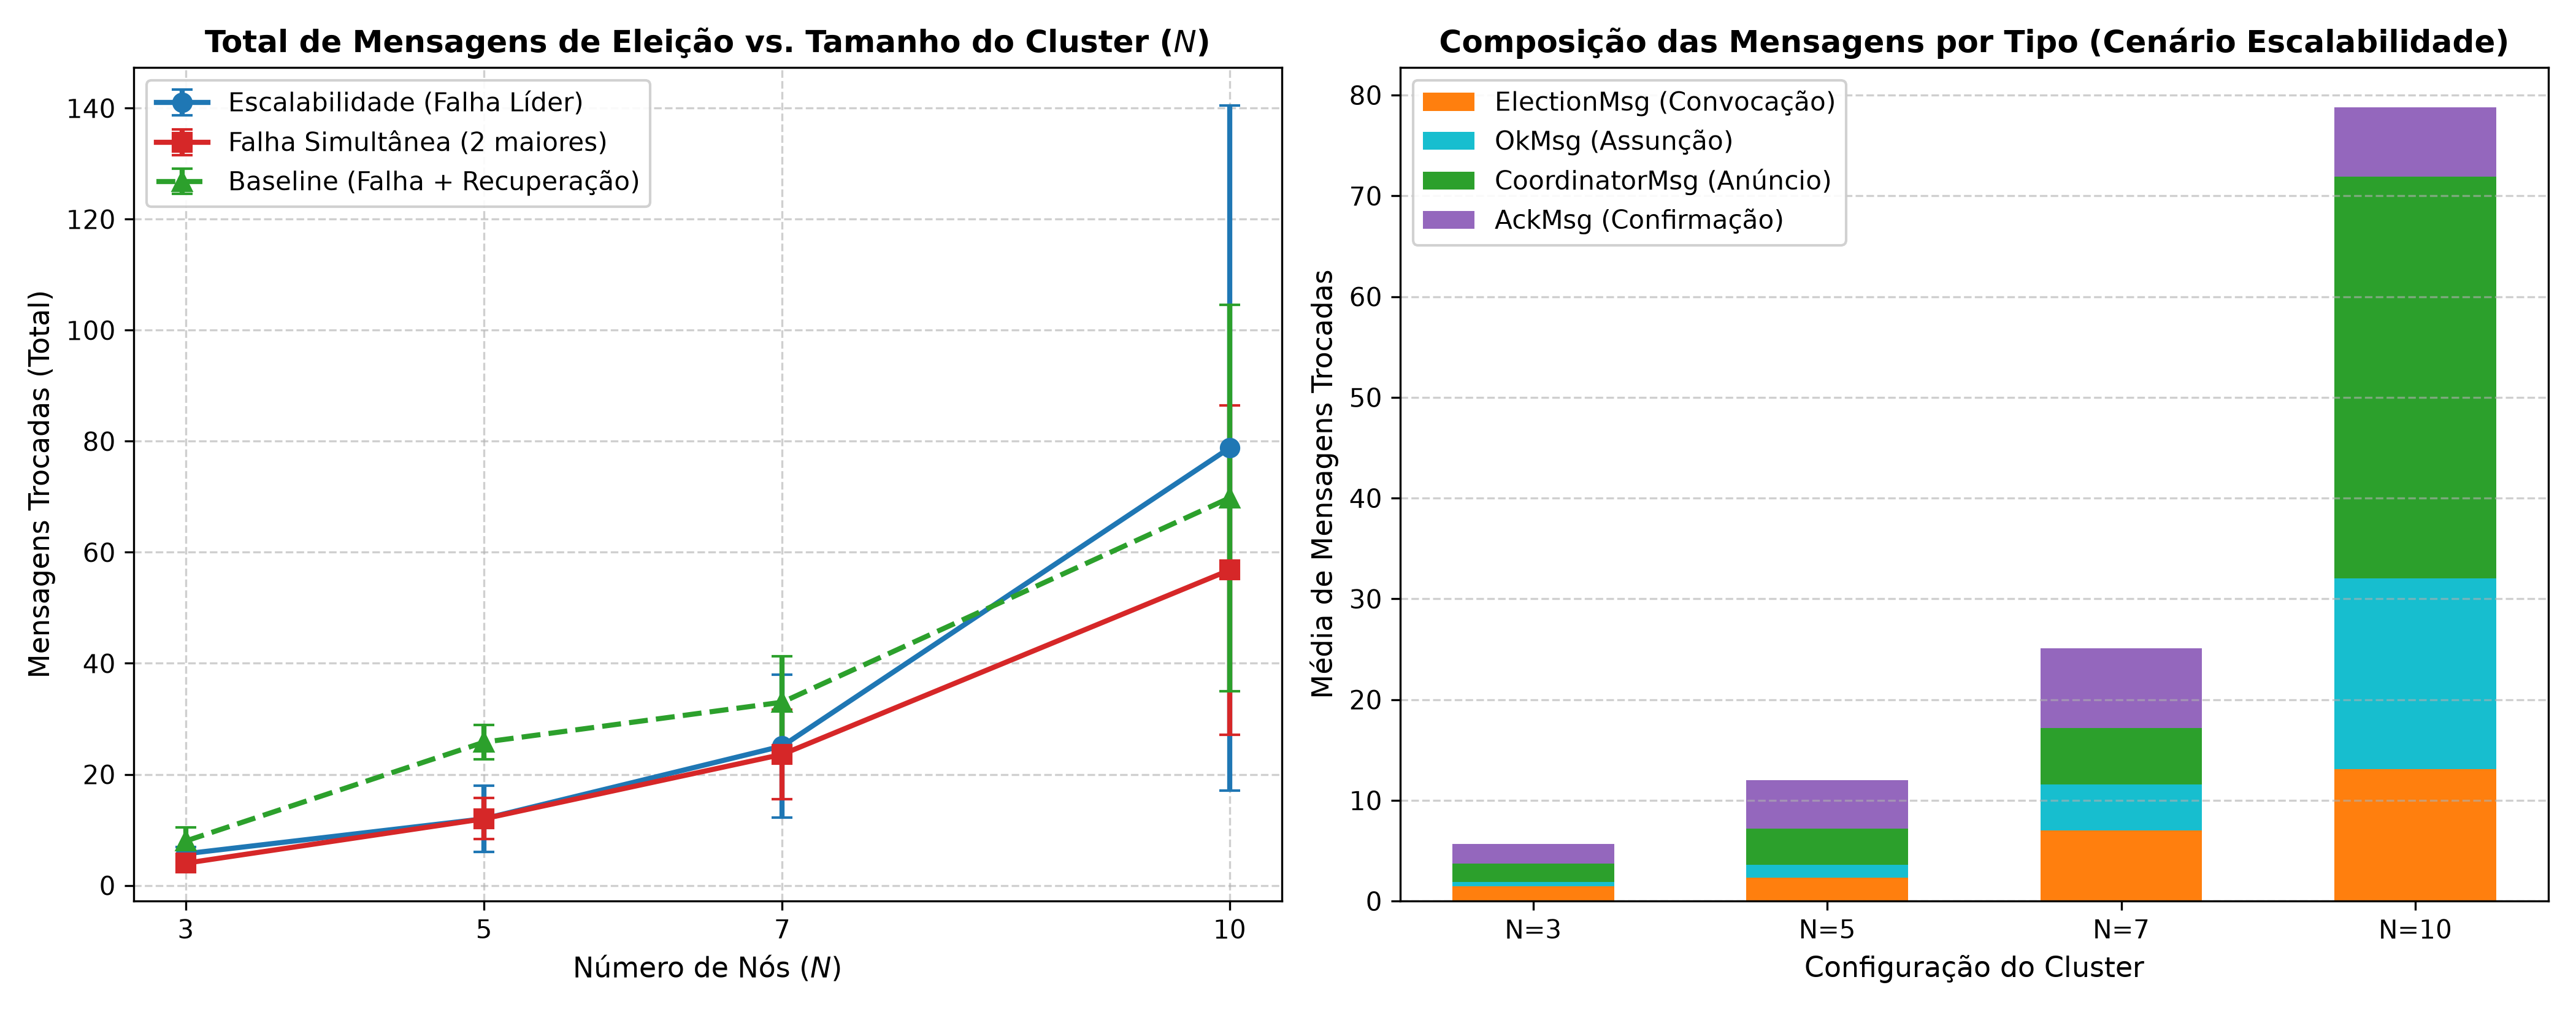
\includegraphics[width=\columnwidth]{images/battery_message_scaling.png}
\caption{Crescimento do volume de mensagens trocadas no algoritmo Bully em função do tamanho do cluster ($N \in \{3, 5, 7, 10\}$).}
\label{fig:messages}
\end{figure}

\begin{figure}[!t]
\centering
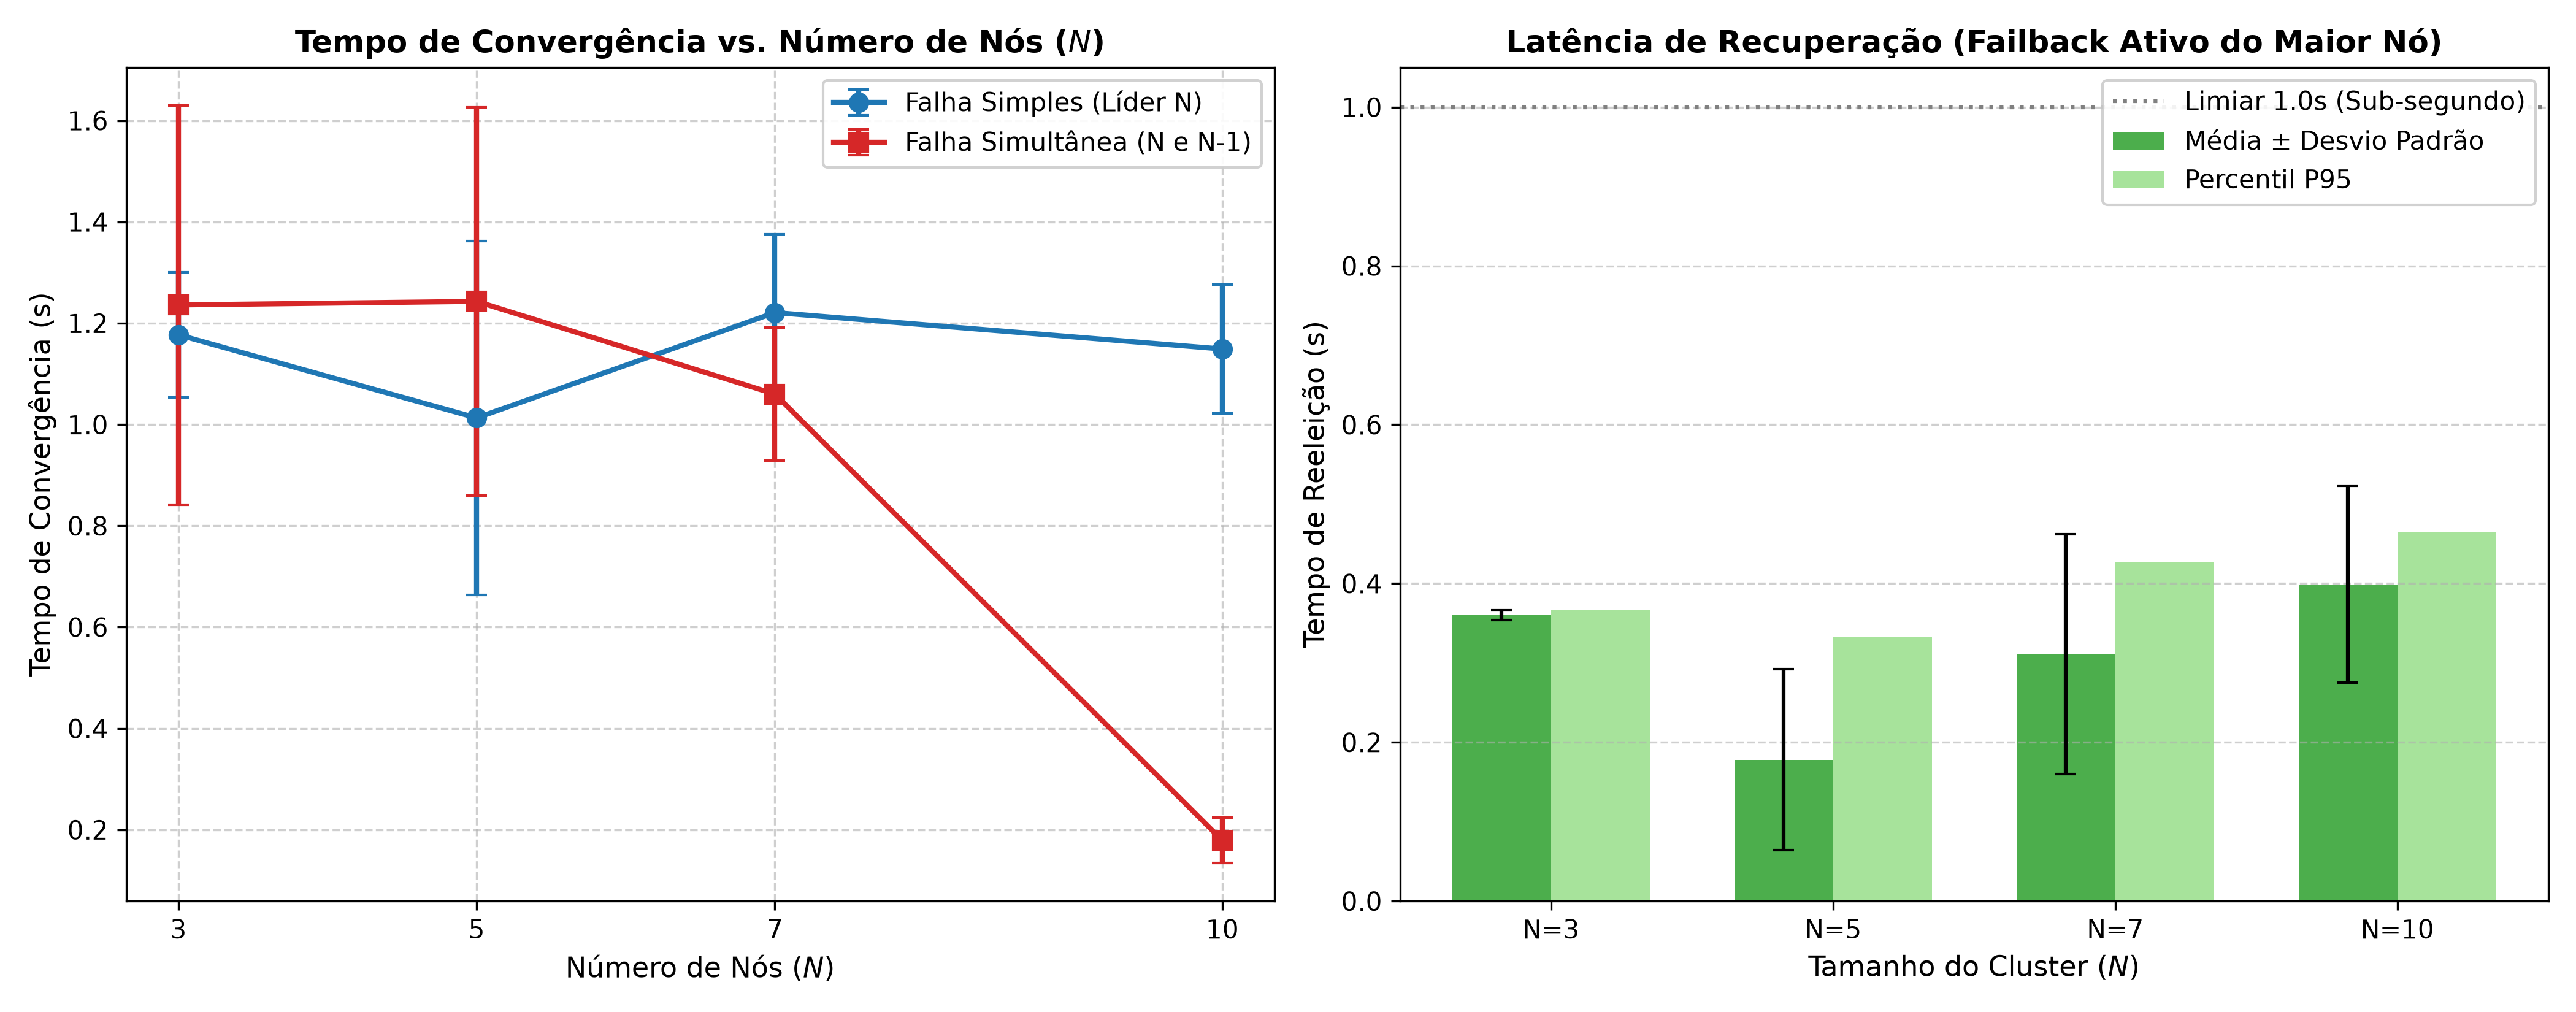
\includegraphics[width=\columnwidth]{images/battery_convergence_scaling.png}
\caption{Latência média de convergência para diferentes cenários e tamanhos de cluster.}
\label{fig:convergence}
\end{figure}

\subsection{Cenários de Falhas Complexas}
No cenário de falhas simultâneas, os contêineres $N$ e $N-1$ foram parados
concomitantemente. Em 100\% das execuções, o nó $N-2$ assumiu com sucesso a
liderança, sem ocorrência de impasses ou bloqueios.

No cenário de falha intermediária ($\lfloor N/2 \rfloor$), nenhuma nova eleição
foi disparada e o coordenador principal permaneceu inalterado e respondendo em
todas as repetições, confirmando a robustez do detector diante de falhas de nós
não coordenadores.

\section{Discussão e Análise}
\label{sec:discussao}

Os testes unitários e as baterias automatizadas em contêineres comprovaram as
propriedades de correção formal definidas para o sistema:
\begin{enumerate}
    \item \textit{Segurança (Safety):} em todos os ensaios, apenas o nó de maior
    identificador ativo proclamou-se coordenador, e mensagens com
    \texttt{election\_id} desatualizado foram descartadas sem corromper o estado;
    \item \textit{Vivacidade (Liveness):} mesmo sob falhas simultâneas dos dois nós
    de maior prioridade, o cluster convergiu para um novo líder dentro do prazo,
    sem travamentos (\textit{deadlocks}) ou oscilações (\textit{livelocks});
    \item \textit{Detecção:} atrasos pontuais inferiores ao limiar de duas
    verificações não causaram eleições indevidas, como demonstrado na estabilidade
    do líder durante o teste de falha intermediária.
\end{enumerate}

\subsection{Complexidade de Mensagens e Inicialização}
A análise experimental confirma o custo de comunicação $\mathcal{O}(N^2)$ inerente
ao algoritmo Bully clássico no pior caso. Observa-se ainda um elevado desvio padrão
no volume de mensagens para $N=10$ (com medições variando entre 22 e 195 mensagens).
Essa alta dispersão é intrínseca à assimetria do protocolo em relação a qual nó
detecta a falha primeiro: se o maior nó sobrevivente ($N-1$) constata a
indisponibilidade antes dos demais, ele contata apenas o líder inativo e declara
vitória com sobrecarga mínima; por outro lado, se um nó subordinado de baixo
identificador detecta a falha, ele convoca todos os superiores, desencadeando a
propagação em cascata e a tempestade quadrática de mensagens prevista teoricamente.

Para mitigar esse impacto durante a subida conjunta do cluster, foi implementada
uma política de inicialização na qual apenas nós com $ID \ge ID_{coord}$ (ou quando
não há coordenador pré-definido) iniciam eleições ativas. Isso reduz o tráfego de
\textit{bootstrapping} para $\mathcal{O}(N)$, reservando a eleição completa para
quando falhas reais forem detectadas.

\subsection{Limitações do Ambiente}
Embora cada nó lógico execute isolado em um contêiner Docker independente, todos os processos residem na mesma máquina física. Essa configuração impõe limitações práticas fundamentais:
\begin{enumerate}
    \item \textbf{Domínio Único de Falha:} Os contêineres compartilham o mesmo hardware e o núcleo do sistema operacional host. Consequentemente, uma falha de hardware ou parada do daemon do Docker encerra simultaneamente 100\% dos nós do sistema, não representando nós com domínios de falha independentes;
    \item \textbf{Canal Virtual e Latência:} A comunicação via rede em ponte (\textit{bridge}) opera inteiramente em memória local do host, apresentando latência sub-milissegúndica e perda de pacotes quase nula. Em redes geograficamente distribuídas (WAN) com enlaces assimétricos e partições de rede (\textit{split-brain}), o algoritmo Bully clássico não garante consenso sem mecanismos de quórum majoritário, sendo recomendadas abordagens baseadas em Paxos ou Raft para tais cenários;
    \item \textbf{Contenção de CPU:} A disputa por ciclos de processamento e agendamento no host durante tempestades de mensagens de eleição pode atrasar o processamento de respostas RPC, tornando indispensável a calibração de \textit{deadlines} e limiares de tolerância a atrasos transitórios.
\end{enumerate}

\section{Conclusão}
\label{sec:conclusao}

Foi implementado e avaliado um sistema distribuído com eleição Bully, detector de
falhas por heartbeat e comunicação gRPC entre processos independentes em contêineres
Docker. A configuração por Docker Compose torna os cenários reprodutíveis,
enquanto os deadlines explícitos e os identificadores de eleição tornam observável
o tratamento de falhas e de mensagens obsoletas.

Os testes e os experimentos confirmaram que o maior nó ativo é escolhido como
coordenador em 100\% dos cenários avaliados. A redução do intervalo de heartbeat
de 3 s para 1 s reduziu o tempo médio de convergência de 4,900 s para 1,186 s.
A extensão para clusters com $N \in \{3, 5, 7, 10\}$ nós confirmou a curvatura
quadrática $\mathcal{O}(N^2)$ de mensagens do algoritmo Bully e demonstrou a
estabilidade do cluster sob falhas simultâneas de múltiplos líderes e falhas
intermediárias.

Como trabalhos futuros, sugere-se a avaliação em redes de longa distância (WAN)
com enlaces assimétricos e a incorporação de mecanismos de quórum majoritário
para mitigar partições de rede (\textit{split-brain}).


\begin{thebibliography}{1}
\bibitem{tanenbaum2023}
M.~van Steen e A.~S.~Tanenbaum, \emph{Distributed Systems}, 4ª~ed.\hskip 1em plus
  0.5em minus 0.4em\relax distributed-systems.net, 2023.
\end{thebibliography}

\appendices
\section{Código da Implementação}
\label{sec:codigo}

O código-fonte e os dados experimentais estão disponíveis no repositório:
\href{https://github.com/RafaelCarro/MC714_Lab02}{https://github.com/RafaelCarro/MC714\_Lab02}.
O vídeo de explicação e demonstração do sistema estará disponível em:
\texttt{[Link do vídeo a ser inserido pós-gravação]}.

Comandos para compilação, execução de testes e reprodução dos ensaios:
\begin{lstlisting}[language=bash]
# 1. Subir cluster base (N=3):
docker compose up --build
# 2. Executar testes unitarios:
docker compose run --rm node1 pytest -q
# 3. Experimento de referencia (N=3):
python3 scripts/run_experiment.py
# 4. Bateria completa e graficos:
python3 scripts/run_test_battery.py --scenario all -n 3 5 7 10 --repetitions 10
python3 scripts/plot_battery.py
\end{lstlisting}

Os arquivos \texttt{experiments/battery\_results.csv} e
\texttt{experiments/battery\_summary.csv} armazenam, respectivamente, as medições
brutas e as métricas consolidadas dos cenários avaliados.

\section{Divisão de Trabalho}
\label{sec:divisao}

Ambos os integrantes participaram da implementação, dos testes, da execução
dos experimentos e da revisão do relatório. Para fins de atribuição, as
responsabilidades principais foram:

\subsection{Rafael Carro Gaudim}
\begin{itemize}
    \item implementação do servidor, do detector de falhas e da eleição;
    \item testes unitários e automação da coleta de métricas;
    \item seções de introdução, arquitetura, resultados e conclusão.
\end{itemize}

\subsection{Douglas Henrique Pereira}
\begin{itemize}
    \item definição do contrato gRPC e configuração do Docker Compose;
    \item análise do modelo do sistema e das propriedades de correção;
    \item seções de algoritmos, experimentos e discussão.
\end{itemize}

\noindent As decisões de projeto, a integração do código e a revisão final
foram realizadas em conjunto.


\end{document}
